\documentclass[a4paper 12pt]{article}
\usepackage[hmargin=1.2in,vmargin=1in]{geometry}
%\usepackage[latin1]{inputenc}
\usepackage{enumerate}
\usepackage{multirow}
\usepackage{url}
\usepackage{array}
\usepackage{bbm}
\usepackage{setspace}
%\usepackage{soul}
%\usepackage[T1]{fontenc}
\usepackage{color}
\usepackage[colorlinks=false,urlcolor=blue]{hyperref}
\usepackage{amsfonts} % Worcester's
\usepackage{appendix} %Added Jan 2012
\usepackage{graphicx,caption}
\usepackage{subcaption}
%\usepackage{authblk}
%\usepackage{setspace}
\usepackage[authoryear,round]{natbib}
\usepackage{endnotes}
\usepackage{amsmath, amssymb,epstopdf,sgame,booktabs}
%\usepackage{mathtools}
\usepackage{ntheorem}
%\usepackage{amssymb,mathrsfs,multirow,sgame,lscape,subfig,enumitem,float,array,booktabs}
\usepackage{amssymb,mathrsfs,multirow,sgame,pdflscape,float,array,booktabs}
%\usepackage[margin=0.75in]{geometry}
%\usepackage[hmargin=0.9in,vmargin=0.75in]{geometry}
%\usepackage{floatrow}
%\usepackage[toc,page]{appendix}
\usepackage{listings}
%\usepackage{authblk}
\usepackage{color} %red, green, blue, yellow, cyan, magenta, black, white
\definecolor{mygreen}{RGB}{28,172,0} % color values Red, Green, Blue
\definecolor{mylilas}{RGB}{170,55,241}
\usepackage{float}
\title{Effect of Tax Cuts on Growth Rates}

\begin{document}

\maketitle

\section{No Labour}

This section derives the model of endogenous growth where there is no labour. 

\subsection{Model Results}

In this model, a tax cut on capital unambiguously increases growth rate/innovation rate. The equation which determines this is
"no arbitrage" condition on innovation expenditure which has the capital tax rate directly featured in it.

\begin{center}
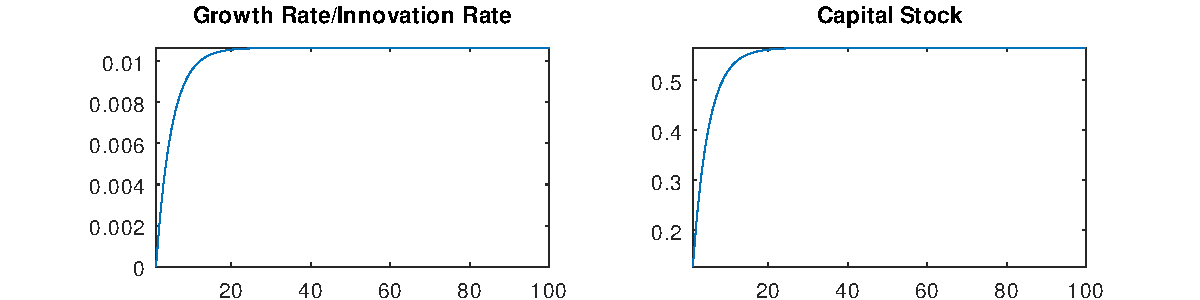
\includegraphics[scale = 0.8]{../product/irfs_nolab.pdf}
\end{center}

\end{document}
